\newcommand{\colorEncabezado}{azulPastelApagado}
\newcommand{\colorTextoEncabezado}{white}
\newcommand{\colorColumnaIzquierda}{azulclaro}

% Columna especial para multicolumns que abarcan las dos últimas columnas con salto de línea automático
\newcolumntype{Y}{>{\hsize=\dimexpr2\hsize+2\tabcolsep+\arrayrulewidth\relax}X}

\section{Personas y Escenarios}


 %PERSONA 1 TUTOR
\subsection{Persona 1: Tutor}
\noindent
\begin{xltabular}{\textwidth}{|p{3.5cm}|X|p{4cm}|}
\hline
\rowcolor{\colorEncabezado}
\multicolumn{3}{|c|}{%
  \color{\colorTextoEncabezado}\textbf{Tutor}%
} \\
\hline

\cellcolor{\colorColumnaIzquierda}\textbf{Nombre}
& Gema Uceda Cabezali
& \multirow{5}{*}{%
  \parbox{3.8cm}{\centering
    \vspace{0.1cm}
    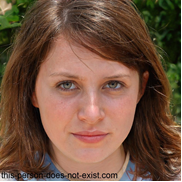
\includegraphics[width=2.6cm, height=2.6cm, keepaspectratio]{img/personas/persona1.png}%
    \vspace{0.1cm}
  }%
} \\
\hhline{|--|~|}

\cellcolor{\colorColumnaIzquierda}\textbf{Edad}
& 37 & \\
\hhline{|--|~|}

\cellcolor{\colorColumnaIzquierda}\textbf{Sexo}
& Mujer & \\
\hhline{|--|~|}

\cellcolor{\colorColumnaIzquierda}\textbf{Discapacidad}
& No tiene & \\
\hhline{|--|~|}

\cellcolor{\colorColumnaIzquierda}\textbf{Educación}
& Estudios universitarios & \\
\hline

\rowcolor{\colorEncabezado}
\multicolumn{3}{|c|}{%
  \color{\colorTextoEncabezado}\textbf{Contexto de uso}%
} \\
\hline

Cuándo
& \multicolumn{2}{Y|}{%
  \small En cualquier momento, utiliza el móvil para tareas cotidianas.%
} \\
\hline

Dónde
& \multicolumn{2}{Y|}{%
  \small En cualquier lugar.%
} \\
\hline

Tipo de ordenador
& \multicolumn{2}{Y|}{%
  \small Principalmente el móvil, aunque también usa el ordenador en el trabajo.%
} \\
\hline

\rowcolor{\colorEncabezado}
\multicolumn{3}{|c|}{%
  \color{\colorTextoEncabezado}\textbf{Misión}%
} \\
\hline

Objetivo
& \multicolumn{2}{Y|}{%
  \small Consultar fácilmente el horario diario de su hijo y ayudarle a organizarlo.%
} \\
\hline

Expectativas
& \multicolumn{2}{Y|}{%
  \small Una interfaz sencilla para programar tareas y consultar sus actividades.%
} \\
\hline

\rowcolor{\colorEncabezado}
\multicolumn{3}{|c|}{%
  \color{\colorTextoEncabezado}\textbf{Motivación}%
} \\
\hline

Urgencia
& \multicolumn{2}{Y|}{%
  \small Cuanto antes.%
} \\
\hline

Deseo
& \multicolumn{2}{Y|}{%
  \small Tranquilidad para ella y para su hijo.%
} \\
\hline

\rowcolor{\colorEncabezado}
\multicolumn{3}{|c|}{%
  \color{\colorTextoEncabezado}\textbf{Actitud hacia la tecnología}%
} \\
\hline

Actitud
& \multicolumn{2}{Y|}{%
  \small Proactiva y capaz de desenvolverse en entornos virtuales nuevos.%
} \\
\hline
\end{xltabular}

\vspace{0.8cm}
%Escenario 1
\noindent
\begin{xltabular}{\textwidth}{|p{3.5cm}|X|p{4cm}|}
\hline
\rowcolor{\colorEncabezado}
\multicolumn{3}{|c|}{%
  \color{\colorTextoEncabezado}\textbf{Escenario 1}%
} \\
\hline

Nombre persona
& Gema Uceda Cabezali
& \multirow{4}{*}{%
  \parbox{3.8cm}{\centering
    \vspace{0.1cm}
    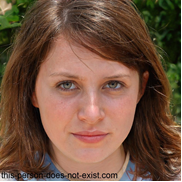
\includegraphics[width=3cm, height=3cm, keepaspectratio]{img/personas/persona1.png}%
    \vspace{0.1cm}
  }%
} \\
\cline{1-2}

Objetivo persona
& \rule{0pt}{2.5cm}Crear una tarea para su hijo & \\
\hline

\rowcolor{\colorEncabezado}
\multicolumn{3}{|c|}{%
  \color{\colorTextoEncabezado}\textbf{Descripción del escenario}%
} \\
\hline

\cellcolor{\colorColumnaIzquierda}\textbf{Descripción}
& \multicolumn{2}{Y|}{%
  \small
  Gema le ha pedido a su hijo que vaya a comprar algo a una
  tienda del vecindario después de salir de clase. Coge el móvil
  y abre la aplicación para añadir la tarea a su agenda.\par\smallskip

  Inicia sesión, accede a la zona de gestión y selecciona el
  perfil de su hijo. Después, elige la opción de añadir una
  tarea, introduce su descripción, la hora de salida del colegio
  y la duración estimada, y confirma la creación.\par\smallskip

  Si no existe ningún conflicto con otras tareas, la aplicación
  incorporará la nueva actividad al calendario. Su hijo podrá
  consultarla al salir de clase.%
} \\
\hline

\end{xltabular}

%Escenario 2
\noindent
\begin{xltabular}{\textwidth}{|p{3.5cm}|X|p{4cm}|}
\hline
\rowcolor{\colorEncabezado}
\multicolumn{3}{|c|}{%
  \color{\colorTextoEncabezado}\textbf{Escenario 2}%
} \\
\hline

Nombre persona
& Gema Uceda Cabezali
& \multirow{4}{*}{%
  \parbox{3.8cm}{\centering
    \vspace{0.1cm}
    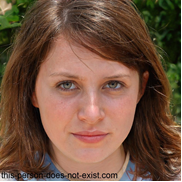
\includegraphics[width=3cm, height=3cm, keepaspectratio]{img/personas/persona1.png}%
    \vspace{0.1cm}
  }%
} \\
\cline{1-2}

Objetivo persona
& \rule{0pt}{2.5cm}Editar una tarea para su hijo & \\
\hline

\rowcolor{\colorEncabezado}
\multicolumn{3}{|c|}{%
  \color{\colorTextoEncabezado}\textbf{Descripción del escenario}%
} \\
\hline

\cellcolor{\colorColumnaIzquierda}\textbf{Descripción}
& \multicolumn{2}{Y|}{%
  \small
  Gema creó una tarea previamente para que su hijo comprara algo en una tienda del vecindario al volver de clases.

En un momento del día, recuerda otra cosa que debe añadir para que su hijo compre, 
se mete en la aplicación logeandose de nuevo y selecciona la tarea previamente añadida. 
Selecciona el botón de edición y modifica la descripción de la tarea. La guarda y ve el cambio reflejado.


} \\
\hline

\end{xltabular}















\newpage

\subsection{Persona 2: Profesor}

 %PERSONA 2 PROFESOR
\noindent
\begin{xltabular}{\textwidth}{|p{3.5cm}|X|p{4cm}|}
\hline
\rowcolor{\colorEncabezado}
\multicolumn{3}{|c|}{%
  \color{\colorTextoEncabezado}\textbf{Profesor}%
} \\
\hline

\cellcolor{\colorColumnaIzquierda}\textbf{Nombre}
& Alejandra Fajardo
& \multirow{5}{*}{%
  \parbox{3.8cm}{\centering
    \vspace{0.1cm}
    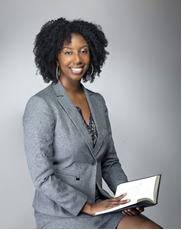
\includegraphics[width=4cm, height=4cm, keepaspectratio]{img/personas/persona2.png}%
    \vspace{0.1cm}
  }%
} \\
\hhline{|--|~|}

\cellcolor{\colorColumnaIzquierda}\textbf{Edad}
& 44 & \\
\hhline{|--|~|}

\cellcolor{\colorColumnaIzquierda}\textbf{Sexo}
& Mujer & \\
\hhline{|--|~|}

\cellcolor{\colorColumnaIzquierda}\textbf{Discapacidad}
& No tiene & \\
\hhline{|--|~|}

\cellcolor{\colorColumnaIzquierda}\textbf{Educación}
& Educación	Universidad – 
Grado en Educación Primaria con mención en Pedagogía Terapéutica (PT)	 & \\
\hline

\rowcolor{\colorEncabezado}
\multicolumn{3}{|c|}{%
  \color{\colorTextoEncabezado}\textbf{Contexto de uso}%
} \\
\hline

Cuándo
& \multicolumn{2}{Y|}{%
  \small Durante la jornada escolar, especialmente al planificar las actividades de la semana, organizar las tareas de los alumnos y consultar qué actividades están previstas para cada día. También puede utilizarlo fuera del horario escolar para preparar y planificar las clases%
} \\
\hline

Dónde
& \multicolumn{2}{Y|}{%
  \small Principalmente en el aula y en la sala de profesores, aunque también puede utilizarlo desde casa para preparar la planificación semanal%
} \\
\hline

Tipo de ordenador
& \multicolumn{2}{Y|}{%
  \small Ordenador portátil o de sobremesa del centro. También podría utilizar ocasionalmente una tableta para consultar rápidamente el calendario durante las clases%
} \\
\hline

\rowcolor{\colorEncabezado}
\multicolumn{3}{|c|}{%
  \color{\colorTextoEncabezado}\textbf{Misión}%
} \\
\hline

Objetivo
& \multicolumn{2}{Y|}{%
  \small Organizar de forma sencilla las actividades, tareas y eventos de sus alumnos mediante un calendario, pudiendo planificar qué debe realizarse cada día y realizar un seguimiento de las actividades pendientes%
} \\
\hline

Expectativas
& \multicolumn{2}{Y|}{%
  \small Espera que la aplicación le permita crear, modificar y consultar tareas fácilmente, organizándolas por alumno y fecha. También espera poder visualizar rápidamente las actividades del día o de la semana y recibir avisos cuando haya tareas o actividades pendientes%
} \\
\hline

\rowcolor{\colorEncabezado}
\multicolumn{3}{|c|}{%
  \color{\colorTextoEncabezado}\textbf{Motivación}%
} \\
\hline

Urgencia
& \multicolumn{2}{Y|}{%
  \small Necesita organizar de forma clara las numerosas actividades y tareas que debe preparar para diferentes alumnos, evitando olvidos y reduciendo el tiempo dedicado a la planificación%
} \\
\hline

Deseo
& \multicolumn{2}{Y|}{%
  \small Quiere tener toda la planificación de sus alumnos organizada en un único lugar, pudiendo saber rápidamente qué tiene que hacer cada día y qué tareas están pendientes para cada alumno%
} \\
\hline

\rowcolor{\colorEncabezado}
\multicolumn{3}{|c|}{%
  \color{\colorTextoEncabezado}\textbf{Actitud hacia la tecnología}%
} \\
\hline

Actitud
& \multicolumn{2}{Y|}{%
  \small Tiene una actitud positiva pero práctica hacia la tecnología. Está dispuesta a utilizar herramientas digitales si le ayudan a organizar mejor su trabajo y ahorrar tiempo. Prefiere aplicaciones sencillas, intuitivas y rápidas, especialmente porque durante la jornada escolar necesita consultar o introducir información sin que esto interfiera demasiado con la atención a los alumnos. Puede sentirse frustrada ante calendarios demasiado complejos o que requieran introducir demasiada información para crear una tarea%
} \\
\hline
\end{xltabular}

\vspace{0.8cm}
%Escenario 1
\noindent
\begin{xltabular}{\textwidth}{|p{3.5cm}|X|p{4cm}|}
\hline
\rowcolor{\colorEncabezado}
\multicolumn{3}{|c|}{%
  \color{\colorTextoEncabezado}\textbf{Escenario 1}%
} \\
\hline

Nombre persona
& Alejandra Fajardo
& \multirow{4}{*}{%
  \parbox{3.8cm}{\centering
    \vspace{0.1cm}
    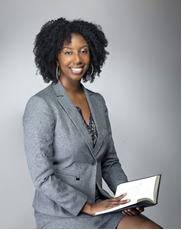
\includegraphics[width=6cm, height=6cm, keepaspectratio]{img/personas/persona2.png}%
    \vspace{0.1cm}
  }%
} \\
\cline{1-2}

Objetivo persona
& \rule{0pt}{2.5cm}Organizar de forma sencilla las actividades, tareas y eventos de sus alumnos mediante un calendario, pudiendo planificar qué debe realizarse cada día y realizar un seguimiento de las actividades pendientes & \\
\hline

\rowcolor{\colorEncabezado}
\multicolumn{3}{|c|}{%
  \color{\colorTextoEncabezado}\textbf{Descripción del escenario}%
} \\
\hline

\cellcolor{\colorColumnaIzquierda}\textbf{Descripción}
& \multicolumn{2}{Y|}{%
  \small
  Alejandra es profesora en un colegio para niños y niñas con discapacidades funcionales. A primera hora de la mañana recibe el aviso de que la excursión prevista para ese día no podrá realizarse debido a la lluvia. La actividad estaba programada en el calendario del colegio y varios alumnos ya estaban preparados para salir.
Alejandra accede a la aplicación para consultar las actividades previstas para ese día y comprueba qué otras actividades estaban programadas para su grupo. Decide reorganizar la jornada y sustituir la excursión por un taller de música que estaba previsto para la semana siguiente. Desde el calendario consulta también qué aula está disponible y qué otros profesionales estaban asignados a cada actividad.
Antes de comenzar el taller, Alejandra actualiza la planificación del día para que el resto del profesorado pueda conocer el cambio. Además, comprueba las actividades de los próximos días para reorganizar el taller de música y evitar que se produzcan coincidencias. De esta forma, consigue adaptar rápidamente la jornada a una situación imprevista y mantiene a todo el equipo informado.
%
} \\
\hline

\end{xltabular}










\newpage

\subsection{Persona 3: Estudiante con visibilidad reducida}

 %PERSONA 3 ESTUDIANTE CON VISIBILIDAD REDUCIDA
\noindent
\begin{xltabular}{\textwidth}{|p{3.5cm}|X|p{4cm}|}
\hline
\rowcolor{\colorEncabezado}
\multicolumn{3}{|c|}{%
  \color{\colorTextoEncabezado}\textbf{ESTUDIANTE CON VISIBILIDAD REDUCIDA}%
} \\
\hline

\cellcolor{\colorColumnaIzquierda}\textbf{Nombre}
& Manuel García
& \multirow{5}{*}{%
  \parbox{3.8cm}{\centering
    \vspace{0.1cm}
    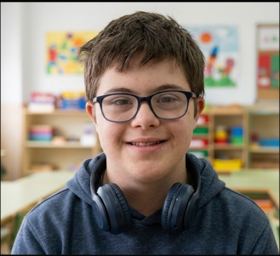
\includegraphics[width=4cm, height=4cm, keepaspectratio]{img/personas/persona3.png}%
    \vspace{0.1cm}
  }%
} \\
\hhline{|--|~|}

\cellcolor{\colorColumnaIzquierda}\textbf{Edad}
& 14 & \\
\hhline{|--|~|}

\cellcolor{\colorColumnaIzquierda}\textbf{Sexo}
& Hombre & \\
\hhline{|--|~|}

\cellcolor{\colorColumnaIzquierda}\textbf{Discapacidad}
& Visibilidad reducida & \\
\hhline{|--|~|}

\cellcolor{\colorColumnaIzquierda}\textbf{Educación}
& Alumno de Educación Especial en el Colegio Fundación Purísima Concepción	 & \\
\hline

\rowcolor{\colorEncabezado}
\multicolumn{3}{|c|}{%
  \color{\colorTextoEncabezado}\textbf{Contexto de uso}%
} \\
\hline

Cuándo
& \multicolumn{2}{Y|}{%
  \small  Cuándo	A lo largo de todo el día, tanto en horario escolar para sus encargos como por la tarde para sus aficiones%
} \\
\hline

Dónde
& \multicolumn{2}{Y|}{%
  \small En cualquier espacio del colegio (aulas, pasillos) y en su casa o lugares de ocio (como el cine)%
} \\
\hline

Tipo de ordenador
& \multicolumn{2}{Y|}{%
  \small Una tablet que pueda llevar siempre consigo, configurada con alto contraste y opciones de accesibilidad de audio%
} \\
\hline

\rowcolor{\colorEncabezado}
\multicolumn{3}{|c|}{%
  \color{\colorTextoEncabezado}\textbf{Misión}%
} \\
\hline

Objetivo
& \multicolumn{2}{Y|}{%
  \small Objetivo	Saber qué le toca hacer en cada momento del día (como sus tareas asignadas en el colegio) y poder añadir y organizar sus propias actividades de ocio (cine, escuchar música)%
} \\
\hline

Expectativas
& \multicolumn{2}{Y|}{%
  \small Espera una aplicación muy visual, con botones muy grandes debido a su reducida visión, y que le "hable" para explicarle las cosas utilizando grabaciones de voces humanas reales y amigables, ya que detesta las voces robóticas o sintéticas%
} \\
\hline

\rowcolor{\colorEncabezado}
\multicolumn{3}{|c|}{%
  \color{\colorTextoEncabezado}\textbf{Motivación}%
} \\
\hline

Urgencia
& \multicolumn{2}{Y|}{%
  \small Alta. Depende de la aplicación para estructurar su tiempo, no perderse durante el día y no olvidar las cosas que más le motivan%
} \\
\hline

Deseo
& \multicolumn{2}{Y|}{%
  \small Entusiasta pero selectivo. Le gusta usar el móvil para escuchar música y cosas de cine, pero se frustra e ignora las aplicaciones si tienen texto pequeño, poco contraste o voces artificiales que le resultan desagradables al oído%
} \\
\hline

\rowcolor{\colorEncabezado}
\multicolumn{3}{|c|}{%
  \color{\colorTextoEncabezado}\textbf{Actitud hacia la tecnología}%
} \\
\hline

Actitud
& \multicolumn{2}{Y|}{%
  \small Proactivo, como chico de su generación está familiarizado con la tecnología y entiende de forma rápida siempre que tenga una interfaz accesible y sencilla %
} \\
\hline
\end{xltabular}

\vspace{0.8cm}
\newpage
%Escenario 1
\noindent
\begin{xltabular}{\textwidth}{|p{3.5cm}|X|p{4cm}|}
\hline
\rowcolor{\colorEncabezado}
\multicolumn{3}{|c|}{%
  \color{\colorTextoEncabezado}\textbf{Escenario 1}%
} \\
\hline

Nombre persona
& Manuel García
& \multirow{4}{*}{%
  \parbox{3.8cm}{\centering
    \vspace{0.1cm}
    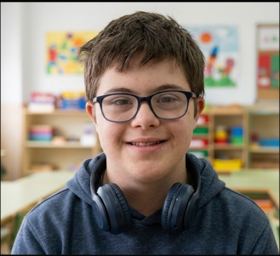
\includegraphics[width=5cm, height=5cm, keepaspectratio]{img/personas/persona3.png}%
    \vspace{0.1cm}
  }%
} \\
\cline{1-2}

Objetivo persona
& \rule{0pt}{2.5cm}Ejercer de embajador del centro enseñando los espacios a personas externas sin desorientarse ni olvidar el recorrido & \\
\hline

\rowcolor{\colorEncabezado}
\multicolumn{3}{|c|}{%
  \color{\colorTextoEncabezado}\textbf{Descripción del escenario}%
} \\
\hline

\cellcolor{\colorColumnaIzquierda}\textbf{Descripción}
& \multicolumn{2}{Y|}{%
  \small
  Es martes por la mañana. Los profesores han asignado a Manuel la tarea de "Guía de visita". Manuel saca su tablet y abre su agenda personalizada. Debido a su visión reducida, la pantalla principal está configurada con fondo negro y un pictograma amarillo muy grande y contrastado que representa una visita.
Manuel pulsa el botón grande de la tarea. Al instante, la aplicación reproduce un audio con la voz natural y cariñosa de su tutora: "¡Hola Manuel! Hoy eres nuestro embajador. Primer paso: llévalos al taller de reprografía". Manuel se siente seguro y guía a los visitantes por el pasillo. Una vez llegan al taller, Manuel saca el móvil y pulsa un botón gigante de confirmación en la pantalla para marcar el fin de ese paso.
La aplicación avanza al siguiente paso y reproduce un nuevo audio, de nuevo con voz humana, indicándole el siguiente destino de la visita. El reloj temporal accesible está oculto en su perfil para que no se ponga nervioso con el paso del tiempo. Al terminar la ruta, Manuel confirma la finalización total de la tarea y la aplicación reproduce el fragmento de su canción favorita a modo de recompensa. Manuel se siente orgulloso de haber hecho un buen trabajo por sí mismo.
%
} \\
\hline

\end{xltabular}





\vspace{0.8cm}
%Escenario 2
\noindent
\begin{xltabular}{\textwidth}{|p{3.5cm}|X|p{4cm}|}
\hline
\rowcolor{\colorEncabezado}
\multicolumn{3}{|c|}{%
  \color{\colorTextoEncabezado}\textbf{Escenario 2}%
} \\
\hline

Nombre persona
& Manuel García
& \multirow{4}{*}{%
  \parbox{3.8cm}{\centering
    \vspace{0.1cm}
    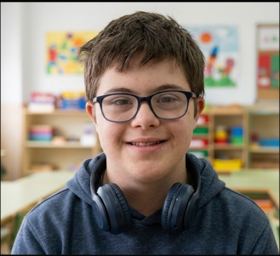
\includegraphics[width=5cm, height=5cm, keepaspectratio]{img/personas/persona3.png}%
    \vspace{0.1cm}
  }%
} \\
\cline{1-2}

Objetivo persona
& \rule{0pt}{2.5cm}Objetivo persona	Crear una tarea personal en su agenda para no olvidar el estreno de una película cuya banda sonora está deseando escuchar & \\
\hline

\rowcolor{\colorEncabezado}
\multicolumn{3}{|c|}{%
  \color{\colorTextoEncabezado}\textbf{Descripción del escenario}%
} \\
\hline

\cellcolor{\colorColumnaIzquierda}\textbf{Descripción}
& \multicolumn{2}{Y|}{%
  \small
  Es miércoles por la tarde y Manuel está en el sofá de su casa. Acaba de ver en la televisión el anuncio de una nueva película de aventuras que se estrena este viernes, y la música del tráiler le ha encantado. Sabe que quiere ir, así que coge su tablet para crear una tarea personal.
Abre la aplicación web y, navegando por su menú adaptado con letras muy grandes, selecciona la opción para añadir una nueva actividad. En lugar de tener que escribir con un teclado pequeño que apenas puede ver, Manuel utiliza un botón de grabación y dice en voz alta: "Ir al cine". El sistema reconoce la instrucción y le pide asignar una imagen. Manuel selecciona un pictograma grande de unas palomitas.
Para la descripción de la tarea, en vez de introducir texto, la aplicación le da la opción de grabar un audio descriptivo en un formato accesible para él. Manuel pulsa el botón de grabar y tararea emocionado un trozo de la canción del anuncio, añadiendo con su propia voz natural: "¡Peli nueva de aventuras!". Finalmente, configura la hora de inicio y fin para el viernes por la tarde. La tarea queda guardada en su agenda semanal y Manuel sonríe sabiendo que el viernes su tablet le avisará con su propia voz de que es la hora de ir al cine.
%
} \\
\hline

\end{xltabular}














\newpage

\subsection{Persona 4: Administrativa}

 %PERSONA 4 ADMINISTRATIVA
\noindent
\begin{xltabular}{\textwidth}{|p{3.5cm}|X|p{4cm}|}
\hline
\rowcolor{\colorEncabezado}
\multicolumn{3}{|c|}{%
  \color{\colorTextoEncabezado}\textbf{ADMINISTRATIVA}%
} \\
\hline

\cellcolor{\colorColumnaIzquierda}\textbf{Nombre}
& Carmen Ruiz
& \multirow{5}{*}{%
  \parbox{3.8cm}{\centering
    \vspace{0.1cm}
    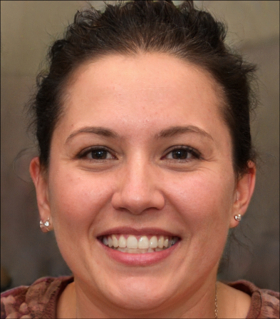
\includegraphics[width=3.8cm, height=3.8cm, keepaspectratio]{img/personas/persona4.png}%
    \vspace{0.1cm}
  }%
} \\
\hhline{|--|~|}

\cellcolor{\colorColumnaIzquierda}\textbf{Edad}
& 43 & \\
\hhline{|--|~|}

\cellcolor{\colorColumnaIzquierda}\textbf{Sexo}
& Mujer & \\
\hhline{|--|~|}

\cellcolor{\colorColumnaIzquierda}\textbf{Discapacidad}
& No tiene & \\
\hhline{|--|~|}

\cellcolor{\colorColumnaIzquierda}\textbf{Educación}
&Personal de Administración y Servicios (PAS) / Técnico en Gestión Administrativa	 & \\
\hline

\rowcolor{\colorEncabezado}
\multicolumn{3}{|c|}{%
  \color{\colorTextoEncabezado}\textbf{Contexto de uso}%
} \\
\hline

Cuándo
& \multicolumn{2}{Y|}{%
  \small  Cuándo	Principalmente al inicio del curso escolar (o de la implantación del sistema) para realizar la carga de datos masiva, y de forma esporádica durante el curso para gestionar nuevas altas, bajas o reasignaciones.%
} \\
\hline

Dónde
& \multicolumn{2}{Y|}{%
  \small En las instalaciones del Colegio de Educación Especial de la Fundación Purísima Concepción, desde un despacho o secretaría.%
} \\
\hline

Tipo de ordenador
& \multicolumn{2}{Y|}{%
  \small Tipo de ordenador	Ordenador de sobremesa del centro educativo o portátil de trabajo.%
} \\
\hline

\rowcolor{\colorEncabezado}
\multicolumn{3}{|c|}{%
  \color{\colorTextoEncabezado}\textbf{Misión}%
} \\
\hline

Objetivo
& \multicolumn{2}{Y|}{%
  \small Crear las cuentas de acceso de todos los usuarios de la plataforma: unos 100-150 estudiantes, además de profesores y tutores. Su labor principal es establecer las relaciones en el sistema, asignando qué estudiantes corresponden a cada profesor y a cada familiar para que ellos gestionen el resto.%
} \\
\hline

Expectativas
& \multicolumn{2}{Y|}{%
  \small Espera encontrar un panel de administración robusto, rápido e intuitivo que le permita gestionar este volumen de usuarios de forma eficiente y sin errores, garantizando que los profesores y estudiantes puedan acceder sin problemas para personalizar sus agendas%
} \\
\hline

\rowcolor{\colorEncabezado}
\multicolumn{3}{|c|}{%
  \color{\colorTextoEncabezado}\textbf{Motivación}%
} \\
\hline

Urgencia
& \multicolumn{2}{Y|}{%
  \small Media. En el colegio tienen una agenda física ya hecha desde hace unos años, pero una aplicación web facilita la logística y sería más amigable con el medio ambiente%
} \\
\hline

Deseo
& \multicolumn{2}{Y|}{%
  \small Desea que la fase de implantación tecnológica sea un éxito y estructurar correctamente la base de usuarios para facilitar la autonomía de los alumnos del Programa de Transición a la Vida Adulta (PTVAL) y el trabajo de los docentes%
} \\
\hline

\rowcolor{\colorEncabezado}
\multicolumn{3}{|c|}{%
  \color{\colorTextoEncabezado}\textbf{Actitud hacia la tecnología}%
} \\
\hline

Actitud
& \multicolumn{2}{Y|}{%
  \small Pragmática y centrada en la eficiencia. Al tener que manejar el registro de unas 100-150 personas, valora por encima de todo las interfaces claras, sin pasos innecesarios, que no le hagan perder tiempo y le eviten incidencias técnicas de acceso con los padres y profesores %
} \\
\hline
\end{xltabular}

\vspace{0.8cm}
\newpage
%Escenario 1
\noindent
\begin{xltabular}{\textwidth}{|p{3.5cm}|X|p{4cm}|}
\hline
\rowcolor{\colorEncabezado}
\multicolumn{3}{|c|}{%
  \color{\colorTextoEncabezado}\textbf{Escenario 1}%
} \\
\hline

Nombre persona
& Carmen Ruiz
& \multirow{4}{*}{%
  \parbox{3.8cm}{\centering
    \vspace{0.1cm}
    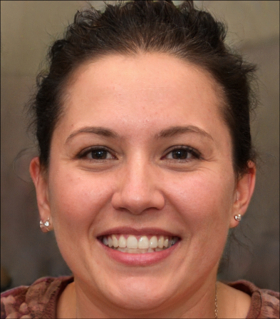
\includegraphics[width=5.5cm, height=5.5cm, keepaspectratio]{img/personas/persona4.png}%
    \vspace{0.1cm}
  }%
} \\
\cline{1-2}

Objetivo persona
& \rule{0pt}{2.5cm} Registrar las cuentas de los estudiantes, profesores y familiares, y vincular a cada estudiante con su tutor y su familia correspondiente para que puedan empezar a usar la aplicación web& \\
\hline

\rowcolor{\colorEncabezado}
\multicolumn{3}{|c|}{%
  \color{\colorTextoEncabezado}\textbf{Descripción del escenario}%
} \\
\hline

\cellcolor{\colorColumnaIzquierda}\textbf{Descripción}
& \multicolumn{2}{Y|}{%
  \small
  Es la primera semana de septiembre en el Colegio de Educación Especial Fundación Purísima Concepción. Carmen, sentada frente al ordenador de secretaría, recibe el listado definitivo de matriculaciones para el nuevo curso. Este año, el centro ha decidido dar el salto y sustituir la tradicional agenda física por la nueva aplicación web, una decisión que a Carmen le motiva porque facilitará la logística diaria y es mucho más respetuosa con el medio ambiente.
Sabe que tiene que registrar a algo más de 100 alumnos, además de a sus profesores y familiares, por lo que entra a la plataforma con su cuenta de administrador con la intención de dejarlo todo listo antes del primer día de clases. Navega al panel de gestión y comienza a introducir los datos. La aplicación le permite ir creando las cuentas de los estudiantes y, en el mismo flujo de trabajo, asignarles quién será su profesor y qué familiares tendrán acceso a su perfil.
A mitad del proceso, el teléfono de secretaría suena; es un padre haciendo una consulta administrativa. Carmen atiende la llamada y, al volver a la pantalla, agradece que el sistema sea claro y le permita retomar el registro exactamente donde lo dejó sin perder la información. Una vez finalizada la carga de todos los usuarios, Carmen pulsa un botón para enviar de forma masiva las credenciales de acceso a los correos de los profesores y los padres. Respira aliviada al ver que el proceso ha sido fluido y sin bloqueos técnicos; ahora el sistema está preparado para que cada familia y profesor entre a personalizar las agendas de sus respectivos alumnos%

} \\
\hline

\end{xltabular}




\newpage

\subsection{Persona 5: Estudiante con discapacidad intelectual}

 %PERSONA 5 ESTUDIANTE CON DISCAPACIDAD INTELECTUAL
\noindent
\begin{xltabular}{\textwidth}{|p{3.5cm}|X|p{4cm}|}
\hline
\rowcolor{\colorEncabezado}
\multicolumn{3}{|c|}{%
  \color{\colorTextoEncabezado}\textbf{ESTUDIANTE CON DISCAPACIDAD INTELECTUAL}%
} \\
\hline

\cellcolor{\colorColumnaIzquierda}\textbf{Nombre}
& Daniela Martín
& \multirow{5}{*}{%
  \parbox{3.8cm}{\centering
    \vspace{0.1cm}
    
\includegraphics[width=3.8cm, height=3.8cm, keepaspectratio]{img/personas/persona5.png}%
    \vspace{0.1cm}
  }%
} \\
\hhline{|--|~|}

\cellcolor{\colorColumnaIzquierda}\textbf{Edad}
& 19 & \\
\hhline{|--|~|}

\cellcolor{\colorColumnaIzquierda}\textbf{Sexo}
& Mujer & \\
\hhline{|--|~|}

\cellcolor{\colorColumnaIzquierda}\textbf{Discapacidad}
& Discapacidad Intelectual & \\
\hhline{|--|~|}

\cellcolor{\colorColumnaIzquierda}\textbf{Educación}
&	Estudiante del Programa de Transición a la Vida Adulta (PTVAL) & \\
\hline

\rowcolor{\colorEncabezado}
\multicolumn{3}{|c|}{%
  \color{\colorTextoEncabezado}\textbf{Contexto de uso}%
} \\
\hline

Cuándo
& \multicolumn{2}{Y|}{%
  \small Utiliza la aplicación a lo largo del día para consultar las actividades que tiene programadas, tanto en el centro, al comenzar la jornada, antes de realizar una tarea o al terminarla, como en casa, para consultar sus actividades personales y las tareas programadas  %
} \\
\hline

Dónde
& \multicolumn{2}{Y|}{%
  \small En el centro educativo y en casa%
} \\
\hline

Tipo de ordenador
& \multicolumn{2}{Y|}{%
  \small Teléfono móvil o Tablet%
} \\
\hline

\rowcolor{\colorEncabezado}
\multicolumn{3}{|c|}{%
  \color{\colorTextoEncabezado}\textbf{Misión}%
} \\
\hline

Objetivo
& \multicolumn{2}{Y|}{%
  \small Consultar y seguir su agenda personalizada para saber qué actividades tiene programadas, cuándo debe realizarlas, qué pasos debe seguir y cuánto durará cada actividad, tanto en el centro como en su vida cotidiana%
} \\
\hline

Expectativas
& \multicolumn{2}{Y|}{%
  \small Espera encontrar una agenda sencilla, clara y adaptada a sus necesidades, que le permita identificar fácilmente cada actividad mediante imágenes, saber cuándo comienza y termina y recibir avisos que le ayuden a anticipar los cambios. También espera poder consultar instrucciones accesibles mediante texto, audio, o secuencias de imágenes cuando necesite ayuda para realizar una tarea%
} \\
\hline

\rowcolor{\colorEncabezado}
\multicolumn{3}{|c|}{%
  \color{\colorTextoEncabezado}\textbf{Motivación}%
} \\
\hline

Urgencia
& \multicolumn{2}{Y|}{%
  \small Urgencia	Necesita consultar la agenda durante el día, especialmente cuando comienza una actividad, cuando termina una tarea o cuando necesita saber qué tiene que hacer a continuación%
} \\
\hline

Deseo
& \multicolumn{2}{Y|}{%
  \small Quiere saber con antelación qué va a hacer y cuánto tiempo tiene para cada actividad, para sentirse seguro y poder realizar sus tareas con mayor autonomía, reduciendo la necesidad de preguntar continuamente a otras personas%
} \\
\hline

\rowcolor{\colorEncabezado}
\multicolumn{3}{|c|}{%
  \color{\colorTextoEncabezado}\textbf{Actitud hacia la tecnología}%
} \\
\hline

Actitud
& \multicolumn{2}{Y|}{%
  \small  Precavida, ya que requiere aplicaciones sencillas que tengan interfaces intuitivas, con pocos elementos, imágenes, botones y texto grandes %
} \\
\hline
\end{xltabular}

\vspace{0.8cm}
\newpage
%Escenario 1
\noindent
\begin{xltabular}{\textwidth}{|p{3.5cm}|X|p{4cm}|}
\hline
\rowcolor{\colorEncabezado}
\multicolumn{3}{|c|}{%
  \color{\colorTextoEncabezado}\textbf{Escenario 1}%
} \\
\hline

Nombre persona
& Daniela Martín
& \multirow{4}{*}{%
  \parbox{3.8cm}{\centering
    \vspace{0.1cm}
    
\includegraphics[width=4.5cm, height=4.5cm, keepaspectratio]{img/personas/persona5.png}%
    \vspace{0.1cm}
  }%
} \\
\cline{1-2}

Objetivo persona
& \rule{0pt}{2.5cm} Saber qué actividades tiene programadas, cuándo debe realizarlas y qué pasos debe seguir para poder realizarlas de forma autónoma y con seguridad en el centro& \\
\hline

\rowcolor{\colorEncabezado}
\multicolumn{3}{|c|}{%
  \color{\colorTextoEncabezado}\textbf{Descripción del escenario}%
} \\
\hline

\cellcolor{\colorColumnaIzquierda}\textbf{Descripción}
& \multicolumn{2}{Y|}{%
  \small
  Daniela comienza una mañana de su jornada en el centro y consulta su agenda para conocer las actividades programadas para ese día. Entre ellas encuentra una tarea de reprografía añadida previamente por el profesor, donde puede visualizar el nombre de la actividad, la imagen asociada y el horario en el que debe realizarla.
Cuando llega la hora indicada, la aplicación la avisa de que debe comenzar. Daniela consulta la tarea y visualiza una secuencia de imágenes que le indica los pasos que debe seguir. Primero debe recoger un material en un aula, después llevarlo al taller de reprografía para realizar las copias y finalmente volver al aula para repartir el material.
Daniela confirma el inicio de la tarea y comienza a realizarla. Mientras trabaja, puede consultar el tiempo restante mediante el reloj temporal, que tiene configurado en su perfil. Las imágenes le indican qué debe hacer a continuación, lo que le permite realizar la actividad con mayor autonomía. Además, puede ir marcando las tareas que ha ido realizando conforme va avanzando en la actividad.
Una vez finalizada la actividad, Daniela la marca como completada y la aplicación actualiza automáticamente su agenda, mostrando la siguiente actividad programada para que pueda continuar su jornada sin depender de las indicaciones constantes del tutor
%

} \\
\hline

\end{xltabular}




\vspace{0.8cm}
\newpage
%Escenario 2
\noindent
\begin{xltabular}{\textwidth}{|p{3.5cm}|X|p{4cm}|}
\hline
\rowcolor{\colorEncabezado}
\multicolumn{3}{|c|}{%
  \color{\colorTextoEncabezado}\textbf{Escenario 2}%
} \\
\hline

Nombre persona
& Daniela Martín
& \multirow{4}{*}{%
  \parbox{3.8cm}{\centering
    \vspace{0.1cm}
    
\includegraphics[width=4.5cm, height=4.5cm, keepaspectratio]{img/personas/persona5.png}%
    \vspace{0.1cm}
  }%
} \\
\cline{1-2}

Objetivo persona
& \rule{0pt}{2.5cm} Saber qué actividades tiene programadas, cuándo debe realizarlas y qué pasos debe seguir para poder realizarlas de forma autónoma y con seguridad en casa& \\
\hline

\rowcolor{\colorEncabezado}
\multicolumn{3}{|c|}{%
  \color{\colorTextoEncabezado}\textbf{Descripción del escenario}%
} \\
\hline

\cellcolor{\colorColumnaIzquierda}\textbf{Descripción}
& \multicolumn{2}{Y|}{%
  \small
  Daniela ha finalizado su jornada en el centro y al volver a casa vuelve a consultar su agenda para ver las actividades personales que ella misma o sus padres han añadido, como hacer los deberes, regar las plantas o una quedada con amigos. 
Ese día, Daniela tiene programada a las cinco una quedada con sus amigos en el parque. Sin embargo, cuando llega la hora de realizarla, comienza a llover y Daniela recibe una notificación indicando que la actividad ha sido cancelada por sus padres debido a la lluvia. La aplicación actualiza automáticamente su agenda y le muestra una propuesta alternativa para realizar en casa, como dibujar.
Una vez finalizada la actividad alternativa, Daniela confirma que la ha completado y la aplicación le permite evaluar si le ha gustado. Así, la aplicación registra sus preferencias para ofrecer actividades adaptadas a sus gustos en futuras ocasiones

%

} \\
\hline

\end{xltabular}